\documentclass[
book,
12pt,
oneside,
%twoside
a4paper,
chapter=TITLE,
english,
brazil,
sumario = tradicional,
]{abntex2}
%\documentclass[brazil,display]{elegantbook}

%Pacotes comuns
\usepackage{lmodern} % carrega uma fonte escalável com melhorias em relação à fonte padrão
\usepackage[T1]{fontenc} % define a codificação da fonte a ser usada para a saída em PDF
\usepackage[utf8]{inputenc} % define a codificação dos caracteres de entrada do texto fonte
\usepackage{indentfirst} % faz a indentação do primeiro parágrafo de cada seção
\usepackage{graphicx} % permite a inclusão de imagens no documento
\usepackage{subcaption} % permite a criação de subfiguras e sublegendas
\usepackage{microtype} % faz pequenos ajustes no espaçamento das palavras para melhorar a aparência do documento
\usepackage{multirow} % permite mesclar células em tabelas em múltiplas linhas
\usepackage{lscape} % permite que o documento tenha páginas em modo paisagem
\usepackage[table]{xcolor} % permite colorir células de tabelas
\usepackage{longtable} % permite a criação de tabelas que se estendem por várias páginas
\usepackage{booktabs} % oferece ferramentas para a criação de tabelas com boa aparência
\usepackage{colortbl} % permite colorir tabelas e células de tabela
\usepackage{csvsimple} % permite importar dados de arquivos CSV para tabelas
\usepackage{siunitx} % oferece suporte para unidades de medida e números com formatação específica
\usepackage{geometry} % permite ajustar as margens do documento
\usepackage{multicol} % permite a criação de múltiplas colunas no documento
\usepackage{float} % permite controlar a posição dos elementos flutuantes, como figuras e tabelas
\usepackage{makeidx} % permite criar um índice remissivo para o documento
\usepackage{url} % permite a inclusão de URLs no documento
\usepackage{tikz}

%pacote para teste
\usepackage{lipsum} %gerar textos aleatórios

%pacotes de citações
\usepackage[brazilian, hyperpageref]{backref} %pagigas com as citações na bibli
\usepackage[alf]{abntex2cite} %citações padrão abntex2

% Pacote para personalizar os títulos dos capítulos
\usepackage{titlesec}

% Configurações do pacote titlesec para personalizar os títulos dos capítulos
\titleformat{\chapter}[display]
  {\normalfont\Large\bfseries\filcenter}
  {\chaptertitlename\ \thechapter}
  {0pt}
  {\Large}
\titlespacing*{\chapter}
  {0pt}{-50pt}{40pt}

% Configurações do pacote fancyhdr para personalizar a numeração de página
\usepackage{fancyhdr}
\fancyhf{}
\fancyfoot[R]{\thepage}
\renewcommand{\headrulewidth}{0pt}
\pagestyle{fancy}

%%% ---
%%% Configurações do pacote backref
%%% Usado sem a opção hyperpageref de backref
%%\renewcommand{\backrefpagesname}{Citado na(s) página(s):~}
%%% Texto padrão antes do número das páginas
%%\renewcommand{\backref}{}
%%% Define os textos da citação
%%\renewcommand*{\backrefalt}[4]{
%%	\ifcase #1 %
%%		Nenhuma citação no texto.%
%%	\or
%%		Citado na página #2.%
%%	\else
%%		Citado #1 vezes nas páginas #2.%
%%	\fi}%
%%% ---
%configuração criar um novo tipo de ambiente de flutuação que você pode usar dentro do ambiente multicols em tabela
\newfloat{tab}{htbp}{lot}

% ---
% Informações de dados para CAPA e FOLHA DE ROSTO
% ---
\titulo{DRAFT - Memorial Descritivo Projeto Quadro Ditribuição Terminal }
\autor{Equipe FDDA SOLAR\thanks{\url{www.fddasolar.com.br}}\ \and Valquiria Fenelon Pereira\thanks{suporte@fddasolar.com.br}}
\local{Brasil}
\data{Várzea Alegre - Abril/2023}
% --
% ---
% ---
% compila o indice
% ---
\makeindex
% ---
% ---
% Altera as margens padrões
% ---
\setlrmarginsandblock{3cm}{3cm}{*}
\setulmarginsandblock{3cm}{3cm}{*}
\checkandfixthelayout
% ---
 %---
% Espaçamentos entre linhas e parágrafos
% ---

% O tamanho do parágrafo é dado por:
\setlength{\parindent}{1.3cm}

% Controle do espaçamento entre um parágrafo e outro:
\setlength{\parskip}{0.2cm}  % tente também \onelineskip

% Espaçamento simples
\SingleSpacing
% ----
% Início do documento
% ----

\begin{document}

% Retira espaço extra obsoleto entre as frases.
\frenchspacing

% ----------------------------------------------------------
% ELEMENTOS PRÉ-TEXTUAIS
% ----------------------------------------------------------

%---
%
% Se desejar escrever o artigo em duas colunas, descomente a linha abaixo
% e a linha com o texto ``FIM DE ARTIGO EM DUAS COLUNAS''.
% \twocolumn[    		% INICIO DE ARTIGO EM DUAS COLUNAS
%
%---
% página de titulo


% página de titulo
\maketitle
%%% resumo em português
%%\begin{resumoumacoluna}
%% \vspace{\onelineskip}
%
% %\noindent
% %\textbf{Palavras-chaves}: latex. abntex. editoração de texto.
%%\end{resumoumacoluna}
%% ----------------------------------------------------------
%% ELEMENTOS TEXTUAIS
%% ----------------------------------------------------------
%\textual
% Configura o formato dos capítulos
\chapterstyle{default}
% Configura a numeração de página para iniciar no primeiro capítulo
\pagenumbering{gobble}

%introdução
\chapter{Objetivo}

Este documento tem como objetivo descrever os aspectos técnicos para montagem de quadros  de distribuição elétrico terminal destinado a ligar equipamentos e gabinetes que compões os paineis LED full color publicitário comercializados pela Mundo LED.
Esse projeto  contém memorial de cálculo, esquema unifilar, multifilar, especificações técnicas, dimensionamento dos quadros, e proteção.

\section{Dados gerais do projeto}

Projeto de quadros de distribuição terminal especifico para Paineis LED Full Color, e manual de instalação.
%Contratante: Rafaela – Mundo LED
%Local: Várzea Alegre – CE
%Telefone: (88) 99936-8176
Contratado: 13.517.574 Francisco Danisio Duarte Almeida
Empresa: FDDA SOLAR - CNPJ 13.574.517/0001-36
Enderço: Rua José da Cunha de Menezes, 44  – Zezinho Costa – Várzea Alegre – CE.
Contato: Telefone: 88 9 92921948; email: contato@fddasolar.com.br.
Responsável técnico: \textbf{ Engª Eletricista Drª Valquiria Fenelon Pereira,}
Registro: \textbf{CREA nº 260217282-0.}
Contato: Telefone: 88 9 9240 4981; Email:\textbf{projeto@fddasolar.com.br}.

\begin{table}[ht]
\centering
\begin{tabularx}{\textwidth}{ l X }
\hline
\multicolumn{2}{>{\columncolor{lightgray}}c}{\textbf{Contratante}} \\\hline% deixar esta linha com uma celula e centralizada
Nome & Rafaela \\
Empresa &  Mundo LED \\ 
Local & Várzea Alegre - CE \\ 
Telefone & (88) 99936-8176 \\ \hline
\multicolumn{2}{>{\columncolor{lightgray}}c}{\textbf{Contratado} } \\ \hline %como mesclar as duas celulas e centralizar? e se possivel cinza claro.
Razão Social & 13.517.574 Francisco Danisio Duarte Almeida \\ 
Empresa & FDDA SOLAR - CNPJ 13.574.517/0001-36 \\ 
Endereço & Rua José da Cunha de Menezes, 44 - Zezinho Costa - Várzea Alegre - CE \\ 
Telefone & 88 9 92921948\\
 email & contato@fddasolar.com.br \\ 
Responsável técnico & Engª Eletricista Drª Valquiria Fenelon Pereira \\
Registro & CREA nº 260217282-0 \\ 
Telefone &  88 9 9240 4981 \\
Email    & projeto@fddasolar.com.br \\ \hline
\end{tabularx}
\end{table}





\section{Notas Técnicas Aplicadas}
\begin{description}
\item[NBR 5410] Instalações elétricas de baixa tensão
\item[NR-10] Norma regulamentadora 10 – Segurança em instalações e serviços em eletricidade.
\end{description}

A montagem e/ ou instalação do quadro deve ser realizado por profissional habilitado, qualificado e ou capacitado. 

%%%escopo do projeto´
\chapter{Escopo de Projeto}


O painel de LED pode descrito equipamentos concebidos com o objetivo de receber dados de uma fonte externa fornecendo dados de saída como reprodução de imagens (item 3.3.4 (c) NBR5410:2004), deste modo, ele pode ser classificado como equipamento de tecnologia da informação (ETI).
elaboração e dimensionamento de quadro de distribuição elétrica dedicados a fornecer energia para paineis Full Led com tensão de 127/220V e 220/380 V.


 
\section{Potência dos Modelos de Paineis Full Color}
%tabela com as potências e tamanho de cada modelo
A entrada de energia de cada gabinete é realizado através de fontes de energia. As especifiações de entrada.
\begin{table}[htbp]
\caption{}
\centering
\begin{tabular}{ l c c c c}
\toprule
\multirow{2}{*}{Modelo}& Gabinetes       & 	 		 \multicolumn{3}{c}{Potência (W)} 			 \\ 
\cmidrule{3-5}
                       & Qnt   & \multicolumn{1}{c}{P10} & \multicolumn{1}{c}{P5} & \multicolumn{1}{c}{P8} \\ 
\midrule

Painel 2 X 2           & 4      & 2160 			    & 2736 			& 2520 \\ 
Painel 2 X 3           & 6      & 3240 				& 4104 			& 3780 \\ 
Painel 3 X 2           & 6      & 3240 				& 4104 			& 3780 \\ 
Painel 3 X 3           & 9      & 4860 				& 6156 			& 5670 \\ 
Painel 4 X 2           & 8      & 4320 				& 5472 			& 5040 \\ 
Painel 4 X 3           & 12     & 6480 				& 8208 			& 7560 \\ 
Painel 4 X 4           & 16     & 8640 				& 10944 		& 10080 \\
Painel 5 X 2		 & 10 		& 5400 				& 6840 			& 6300 \\ 
Painel 5 X 3 			& 15 	& 8100 				& 10260 		& 9450 \\
Painel 6 X 2 			& 12 	& 6480 				& 8208 			& 7560 \\ 
Painel 7 X 3 			& 21 	& 11340 			& 14364 		& 13230 \\ 
Painel 9 X 3 			& 27 	& 14580 			& 18468 		& 17010 \\ 
Painel 10 X 4 			& 40 	& 21600 			& 27360 		& 25200 \\
\bottomrule
\end{tabular}
\label{tab:pot_Painel}
\end{table}

 
\section{Tecnologia de iluminação LED}
Existe algumas caracteristicas da tecnologia LED que devemos ter atenção. Tal como alguns potenciais restrições que poderemos ter que superar.
\begin{itemize}
\item Corrente de pico potencialmente muito elevada ao ligar.
\item Geração de poluição hamonica
\item Temperatura elevada nas conexões
\item Radiação no espectro azul
\item Piscar quando desligada.
\end{itemize}

Ao ligar uma luminária LED ocorre uma corrente variavel durante o primeiro segundo, a corrente se estabiliza quando atinge a condição de operação nominal. Na partida da luminária pode ser identificado três estados transitórios:
\begin{itemize}
  \item Estado 1: Corrente de pico.
  \item Estado 2: inicialização do driver.
  \item Estado 3: Alimentando a carga LED.
  \end{itemize}  
O estado 4 correponde a condição de operação estacionário. Este estados estão numerados na figura.
\begin{figure}[h]
    \centering
    \includegraphics[width=0.6\textwidth]{image/correntextempo.png}
    %\includegraphics[width=4cm]{image/EtiqAdvQD.pdf}
    \caption{Gráfico Corrente x tempo, da partida de luminária LED retirada}
   \label{fig:bornes}
\end{figure}
Esta caracteristica influencia na escolha do disjuntor. 

\section{Influências externas}

Condições exterior a que o quadro terminal possam estar sujeitos.
Temperatura ambiente
grau de proteção

\section{Tipos de Quadro Terminal}

Existem proteções básicas e obrigatórios segundo as normas, e a proteção mais especifica que podem ser necessárias devido a influências externas, tal como, sensibilidade de equipamento devido a oscilação da rede, partida de motores de indução, etc.
\begin{description}
\item[Obrigatórios] Proteção contra sobrecorrente. Protege contra incêndios, contra sobrecarga e contra curto circuito. Dispositivo utilizado disjuntor.
\item[obrigatório em áreas úmidas] Proteção contra fuga a Terra. Protege contra
\end{description}

No geral um quadro de distribuição elétrica contém:
\begin{list}{•}{•}
\item Dispositivos de proteção: disjuntores termomagnéticos (DTM), interruptores diferenciais (IDR) e dispositivo de proteção contra surtos(DPS);
\item Barramentos de inteligação das fases;
\item Barramento de neutro;
\item Barramento de proteção PE (terra);
\\item Estrutura: composta de caixa metálica, chapa de montagem dos componentes, isoladores, tampa(espelho) e porta com dobradiça.
\end{list}

Para nomear os quadros vamos utilizar o seguinte padrão de código:
\begin{table}[!h]
\begin{tabular}{c  c c l  l l l r l l}
Quadro 		& l x c		& 	 &{y}			& 		&{Pn}			& 			&{yyyV} 	&			&\\

			& 	\vline	& 	  & 	\vline	&		&		\vline	&			&	\vline 		& 	&	Tensão (F-N) 127; 220;  \\
\cline{9-10} 
			& 	\vline	& 	  & 	\vline	&		&		\vline	&			&			&			&	Led 5, 8 ou 10;  \\
\cline{7-10} 
			& 	\vline	& 	  & 	\vline &		&				&			&			&			&	Monofásico (M), Trifásico (T);  \\
\cline{5-10} 
			& 	\vline	& 	  & 			&		&				&			&			&			&	 Qtd gabinetes por linha(l) e coluna (c);  \\
\cline{3-10} 
\end{tabular}
%\caption{Codigo do quadro para qual painel ele serve}
\end{table}
Como exemplo um quadro terminal para o painel full led  P8 4x3 m que será instalado em uma rede com tensão fase neutro (F-N) 127 V e entre fase 220 V (F-F) no modelo trifásico, terá o seguinte código Quadro 4x3T P8 127V
\section{Parâmetros de Projeto}
Parâmetros de projeto comum para todos os quadros
\begin{itemize}
\item Parâmentros de projeto
\item Corrente de curto circuito:  xx A
\item Queda de tensão
\item Fatores de demanda considerados
\item Temperatura ambiente
\end{itemize}
   
   
A corrente de curto circuito de entrada 380V e potencia de transformador 112,5 kVA Icc 4,8 kA, fator de potência 0,7

\section{Dados do montador}
Conforme a NBR IEC 61439-1 os item declarados pelo montador do conjunto %\cite{NormasTecnicas2016}:
\begin{description}
\item[$U_{n}$] tensão nominal do CONJUTO (item 5.2.1) a tensão nominal deve ser ao menos igual à tensão nominal do sistema elétrico.

\item[$U_{e}$] tensão de utilização de um circuito. A tensão nominal de utilização não pode ser inferior à tensão nominal do sistema elétrico ao qual é previsto para ser conectado.
\item[$U_{i}$] tensão nominal de isolamento de um circuito é o valor da tensão para os quais as tensões de ensaio dielétricas e distâncias de escoamento são referidas. $U_{i} \leq U_{n} e U_{i} \leq U_{e}$

\item[$U_{imp}$] Valor de tensão de impulso suportável, caracterizando a cpacidade de suportar a isolação contra sobretensões trnasitórias especificadas. (item 3.8.9.4 da norma ABNT 61439-1 )

\item[$I_{n}$] valor de corrente que o circuito pode conduzir sem que a elevação de temperatura das diferentes partes do CONJUNTO exceda os limites especificados em condições especificas. $I_{nA}$ corrente nominal do CONJUNTO (item 5.3.1); $I_{nc}$ corrente nominal de um circuito (item 5.3.2)
\item[$I_{pk}$] valor de pico de corrente de curto-circuito, que pode ser suportado sob condições especificadas.
\item[$I_{cw}$] valor eficaz da corrente de curta duração, que o circuito pode suportar em condições especificadas, definido em termos de corrente e duração.
\item[$I_{cc}$]valor da corrente de curto-circuito presumida, que o circuito protegido por um dispositivo de proteção contra curto-circuito (DPCC)pode suportar durante o tempo total de funcionamento desse dispositivo nas condições especificadas.
\item[RDF - \textit{Rated Diversity Factor}] valor por unidade de corrente nominal, que os circuitos de saída de um CONJUNTO podem ser carregados de forma contínua e simultânea leando um consideração as influências térmicas mútuas.
\item[$f_{n}$] valor de frequência para o qual um circuito é projetado e para o qual se referem as condições de utilização.A atribuição pode ser por faixa de frequencia ou especificar se é em corrente alternada ou corrente contínua item 3.8.12


\end{description}


 

%descrição técnica
\chapter{Especificações Técnicas}

Os componentes básicos de um quadro de distribuição são:
\begin{itemize}
\item Dispositivos de proteção: disjuntores (DTM), interruptores diferenciais (IDR) e dispositivo de proteção contra surtos (DPS);
\item Barramentos de interligação fase;
\item Barramento de Neutro;
\item Barramento de proteção
\item Estrutura: caixa com porta, chapa de montagem dos componentes, isoladores, tampa espelho.
\end{itemize}




\section{Condutores elétricos}
Os cabos elétricos utilizados nas instalações devem possuir classe de encordoamento no mínimo 5 ou 6, tanto para os circuitos terminais, quanto para o alimentador do quadro de distribuição QGD1, os cabos dos circuitos terminais deverão ser cabos isolados de PVC (450/750V), nas cores preta, azul, vermelho, branco e ou verde) e unipolar em EPR para o alimentador do quando QGD1.
Todos os condutores deverão seguir a NBR NM 247-3 e possuir o selo do inmetro, todas as seções desses condutores estão descritas na tabela de carga de acordo com os seus respectivos circuitos e deverão ser seguidos.
ATENÇÃO A escolha dos cabos devem ser realizadas conforme a Norma 5410.

\section{Disjuntores}
Os disjuntores devem ser de tensão nominal de serviço Ue = 400V ou superior. Seguir as correntes nominais de atuação de sobrecarga conforme indicado em projeto. As correntes de ruptura devem ser de 3kA para os disjuntores de circuitos terminais e 5kA para o disjuntor geral. As curvas de disparo devem seguir conforme indicado na tabela de carga, assim como a escolha da quantidade de pólos.
Todos os disjuntores existentes no projeto devem ser de fabrincantes que possuem o selo do INMETRO de certificação compulsória e os responsáveis pela compra e execução dos materiais deverão utilizadas marcas de confiança e consolidadas no mercado como Schneider, WEG, ABB, Siemens, Steck ou similar. 
Todos os disjuntores deverão seguir as normas:\begin{list}{•}{•}
\item ABNT NBR 5361 - Disjuntores de baixa tensão;
\item ABNT NBR IEC 60947-2 -  Dispositivo de manobra e comando de baixa tensão;
\item ABNT NBR NM 60898 (ou IEC 61009-2-1) – Disjuntores para proteção de sobrecorrentes para instalações domésticas e similares
\end{list}



\begin{table}[htbp]
\centering
\caption{Capacidade de interrupção máxima $I_{cn}$ }

\begin{tabular}{|l|c|c}
%\begin{tabular}{llccccccccc}

& 127/220 V 220/380 V  \\\hline
NBR NM 60898 & 5kA & 3 kA)\\ \hline
NBR IEC 60947-2 & 5kA & 4,5 kA)\\ \hline
\end{tabular}
\label{tab:disjIcn}
\end{table}



\section{IDR – Interruptor diferencial residual}

Dispostivos DR são seccionadores mecânicos projetados para provocar abertura na ocorrência de uma corrente de fuga à terrra. Tem como principal objetivo proteger as pessoas contra os efeitos dos choques elétricos prejudiciais a saúde. De acordo com NBR 5410/2004 item 5.1.3.2.2, seu uso é obrigatório nos circuitos elétricos localizados em áreas molhadas e externa [Siemens 2023].
Sua versão de corrente residual até 30 mA são destinados a principalmente a proteção de pessoas, acima deste valor, são apropriados para a proteção de instalações elétricas. Existe 3 tipos de dispositivos DR:
    1. Tipo AC – detecta correntes residuais alternadas;
    2. Tipo A – detecta correntes residuais alternadas e continua pulsantes.
    3. Tipo B – detecta correntes residuais alternadas, continuas pulsantes e continuas puras[Siemens 2023].
O IDR a ser utilizado deverá ser ligado em série com o disjuntor geral e este deve possuir corrente nominal igual ou superior a corrente nominal do disjuntor termomagnético geral do quadro QDC. O valor de atuação da corrente diferencial do IDR deverá ser de 30mA. O IDR deverá seguir a norma ABNT NBR NM 61008-1 (verificar validade no site da ABNT)
\section{DPS – Dispositivo de proteção contra surtos elétricos}
O DPS utilizado deverá ser do tipo classe II, 175V e 20kA e este deverá ser instalado dentro do quadro de distribuição QGD1. O DPS deverá seguir a norma ABNT NBR IEC 61643-1 (verificar validade no site da ABNT), NBR 5410 e NBR 5419.

\section{Quadro elétrico e acessórios}
    1 O quadro de distribuição deve seguir a norma NBR IEC 60439-1 e NBR 5410.

No quadro deverão estar presentes os seguintes itens:

    2 Tensão nominal: (220/127V)
    3 Corrente de demanda: 34,55A
    4 Capacidade de Curto-circuito: 5kA
    5 Grau de proteção IP adequado e no mínimo IP2X.
    6 Placa de Identificação do quadro contendo nome ou marca do fabricante e tipo ou numero de identificação.

O instalador deverá inserir etiqueta de advertência conforme NBR 5410 no item 6.5.4.10 mostrada abaixo:

5.6.5.2 Quando existir risco de choque elétrico, o dispositivo de seccionamento de emergência deve seccionar todos os condutores vivos, observada a prescrição de 5.6.2.2
Perfil
Canaleta DN
as canaletas DN servem para agrupar, proteger e organizar os fios e cabos dentro do quadro elétrico. São de PVC rígido em conformidade com a Norma Diretiva 2002/95/EC-RoHS

\subsection{Grau de Proteção}
Determina a proteção do quadro metálico quanto a entrada de corpos estranhos e penetração de água por frestas e orificios do quadro. As normas especificam os graus de proteção por código IPXY, onde X indica o grau de proteção quanto à penetreção de corpos sólidos e contatos acidentais. Enquanto que o Y é um número que indica o grau de proteção quanto a penetração de água internamente no quadro quando fechado. 
Os graus de proteção identificados pelas letras IP seguida de dois números que significam (%\citep{Filho2013})

\begin{itemize}
\item \textbf{Primeiro algarismo}
 	\begin{description}
 	\item[0-] sem proteção;
 	\item[1-] corpos estranhos com dimensões acima de 50 mm;
 	\item[2-] corpos estranhos com dimensões acima de 12 mm;
 	\item[3-] corpos estranhos com dimensões acima de 2,5 mm;
 	\item[4-] corpos estranhos com dimensões acima de 1 mm;
 	\item[5-] proteção contra acúmulo de poeira prejudicial ao equipamento;
 	\item[6-] proteção contra penetração de poeira.
 	\end{description}
 	
 \item \textbf{Segundo algarismo}
 
 		\begin{description}
 		\item[0-] sem proteção;
 		\item[1-] pingos de água na vertical;
 		\item[2-] pingos de água até a inclinação de 15° com a vertical;
 		\item[3-] água de chuva até a inclinação de 60° com a vertical;
 		\item[4-] respingos em todas as direções;
 		\item[5-] jatos de água em todas as direções;
 		\item[6-] imersão temporária;
 		\item[7-] imersão;
 		\item[8-] submersão.
 		\end{description}
\end{itemize}



\subsection{Bornes}
Os bornes permitem uma conexão segura quadro a rede e ao Painel. Propocionando flexibilidade, facilidade e rapidez na instalação. Existe três opções de conexão: por parafuso, por mola e plug-in.

\begin{figure}[h]
    \centering
    \includegraphics[width=0.6\textwidth]{image/BORNESIMENS.png}
    %\includegraphics[width=4cm]{image/EtiqAdvQD.pdf}
    \caption{Imagens retirada do catálogo siemens com vários tipos de borne}
   \label{fig:bornes}
\end{figure}
\begin{description}
\item[Borne padrão] utilizado como um conector de passagem, tem disponivel em vários tamanho, cores em geral bege, azul e laranja. Servirão para conectar condutores de fase e neutro de entrada e saída do quadro.
\item[Borne Terra] borne especial para proteção equipotecial, sempre na cor verde-amarela. Por suas caracteristicas, nunca deve ser utilizado como borne de passagem padrão. Ou seja, SOMENTE utilizar como entrada ou saida de aterramento, NUNCA ligar condutores fase ou neutro.
\end{description}
\subsection{Barramentos}
Os barramentos de cobre são indicados para instalações elétricas com o objetivo de fazer a ligação de vários circuitos, de modo mais funcional e seguro.
O barramento fase tipo pente ou pente de conexão ou barramento de alimentação tem modo de montagem horizontal em linha. Serva para ligações monofásicas, bifásicas e trifásicas. Com corrente nominal de 63 A a 130 A, podem ser encontrados com 12, 24 e 57 polos. Tem capa ou terminal isolador apropriado, onde uma peça tem cinco módulos isolador. 
\begin{figure}
\centering
\begin{subfigure}{0.4\textwidth}
	\includegraphics[width=\textwidth]{image/barramentofase.png}
	\caption{Barramento fase tipo pente e seu modo de ligação e respectiva corrente nominal. }
	\label{fig:advQD_1}
\end{subfigure}
\hfill
\begin{subfigure}{0.4\textwidth}
    \includegraphics[width=\textwidth]{image/barramentocapa.png}
    \caption{Capa isolante}
    \label{fig:advQD_2}
\end{subfigure}
\caption{Barramento para fase caracteristicas retirado do catálogo Simens}
\label{fig:advQD}
\end{figure}

\section{Dispositivos de comando}
\subsection{Contatores}
Contatores são elementos de comandos eletromêcanicos, que permite o controle de correntes elevadas por meio de circuitos de baixa corrente. O contator funciona como uma chave eletromagnética, constituido por uma bobina, que quando alimentada, cria um campo eletromagnetico que fecha o circuito, e ao cessar a alimentação da bobina o circuito é aberto. 
%
\begin{figure}[h]
    \centering
    \includegraphics[width=0.6\textwidth]{image/contator_simbolo.png}
    
    \caption{Simbologia do contator. Fonte\cite{Franchi2008}}
   \label{fig:bornes}
\end{figure}

\subsection{Interruptor horário}
Interruptor horário eletrônicos ou interruptor temporizador, permite a programação de horário para ligar e desligar automáticamente, com algumas combinações de frequência diária semanal, como por exemplo, todos os dias, dias úteis, entre outras.
A Figura \ref{fig:esqtemp_1} tem o esquema de ligação para controle automático de luminosos, um sistema por comando direto, e outro com uso de contator necessário para circuitos luminosos com corrente acima de 10 A. Assim como os interruptores a capacidade nominal de o interruptore temporizador é de 10 A.
\begin{figure}
\centering
	\includegraphics[width=\textwidth]{image/esqTemp.png}
	\caption{Esquema multifilar de ligação do controle automático por interruptor temporizador.}
	\label{fig:esqtemp_1}
\end{figure}


\subsection{Relé de Impulso}
Possivel comandar com botão pulsador a distância ou por um ou mais pulsadores, para os esquemas multifilar mostrados nesta seção, considerar a carga de iluminação dentro da capacidade do relé.
 

%calculos básicos
%\chapter{cap}
\chapter{Calculos Básicos}
\label{cap:calculos}
Parametros para calculos
Fator de potência indica quando a energia solicitada da rede está sendo usada de forma útil. \textbf{$FP= cos \phi < 1,0$}
Tipos de linhas método de referência para a capacidade de corrente, \textbf{B1} que equivale a cabos isolados em eletrodutos circulares embutidos ou aparentes, o modo mais comun de instalação considerado até a entrada do quadro.
Do quadro até os gabinetes \textbf{ B2} cabos multipolares.
Numero de condutores carregados, considerando 2 para monofásicos e 3 para trifásicos.
Cabos de cobre 70ºC isolação PVC


\section{Corrente de projeto Ip ou Ib}
Corrente de projeto ($I_{p}$) ou ($I_{b})$ que os condutores devem suportar levando em consideração suas características nominais (Tabela \ref{tab:eqIp}).

\begin{table}[htbp]
\caption{Equações utilizadas para encontrar a corrente nominal de projeto.}
\begin{center}
\begin{tabular}{|c|c|}
\hline
Circuito & Equação \\ \hline
Monofásico (F+N) &\rule{0pt}{12pt} $I_{p}=\frac{P_{n}}{V \cdot \cos \varphi \cdot \eta}$ \rule[-6pt]{0pt}{0pt} \\ \hline
Trifásico (3F+N) & \rule{0pt}{12pt} $I_{p}=\frac{P_{n}}{\sqrt{3} \cdot V \cdot \cos \varphi \cdot \eta}$ \rule[-6pt]{0pt}{0pt} \\ \hline
\end{tabular}
\label{tab:eqIp}
\end{center}
\end{table}
%\begin{table}[htbp]
%\caption{Equações utilizadas para encontrar a corrente nominal de projeto.}
%\begin{tabular}{|c|c|}
%\hline
%Circuito & Equação \\ \hline
%Monofáscio (F+N) & \begin{equation}
%I_{p}=P_{n} over {V cdot cos %varphi cdot %eta}
%\end{equation} \\ \hline
%trifásico (3F+N) & 
%\begin{equation}
%I_{p}=P_{n} over { sqrt{3} cdot V CDOT cos %varphi  cdot %eta}
%\end{equation} \\ \hline
%\end{tabular}
%\label{tab:eqIp}
%\end{table}

%tabela
%Circuito
%Formula
%Monofásico (F + N)
%
%Trifásico (3F + N)
%tabela com formula
%Sendo:
%\begin{equation}
%
%I_{p} = I_{p}  leslant I_{n} leslant I_{z} ; (b) I_{2} leslant 1,45 cdot I_{z}
%
%\end{equation}

%\begin{equation}
%I_{p}=P_{n} over { sqrt{3} cdot V CDOT cos %varphi  cdot %eta}
%\end{equation}


Esquema de distribuição de condutores vivos:
Corrente alternada monofásico a dois condutores F + N (220V ou 127V)
Corrente alternada trifásico a quatro condutores 3F + N (380V ou 220V)

\section{Metodos para dimensionamento de cabos}

 Método de referência para os calculos de capacidade de condução de corrente
B1
Condutores isolados ou cabos unipolares em eletroduto circulares aparaente ou embutido em alvenaria. Tipo de instalação mais comum, considerado para alimentação do QDP (quadro de distribuição do painel).
Esquema de aterramento
A alimentação do quadro de ser composto por uma proteção PE (aterramento), um neutro,  uma fase para monofásica ou três fases para trifásica
Em esquema TN o seccionaento automático visando proteção contra choque elétrico, pode ser usados dispositivos de proteção de sobrecorrente, dispositivos de proteção a corrente diferencial-residual (dispositivo DR), sendo este não é admitido quando usando a variante TN-C.


Pn – Potência elétrica nominal (W);
V – Tensão elétrica entre fase (V);
$\eta$ – Rendimento considerado = 1;
cos $\varpi$ -  fator de potência (considerado = 1)
Numero de condutores carregados:
    • 2 para alimentação de quadro monofásico e circuitos de distribuição;
    • 3 para alimentação de quadro trifásico.
Tabela 2: Capacidade de condução de corrente (A) para metodo B1; condutor de cobre, 70°C, PVC, temperatura ambiente 30°C(ar). Fonte tabela 36 NBR 5410:2004
começo tabela
fim tabela

    Parâmentros de projeto
        Corrente de curto circuito:   A
        Queda de tensão
        Fatores de demanda considerados
        Temperatura ambiente
    • Cálculo de demanda
    • Dimensionamento dos condutores
    • Dimensionamento dos eletrodutos
    • Dimensionamento das proteções
\subsection{ Metodo da queda de tensão}
Para a alimentaçao principal a distancia L dentro do quadro 1,2 m no pior caso Quadro 10x3.  Para alimentação da tomada = 0,95 m. Para os Circuitos L = 5 m


\subsection{Dimensionamento Neutro e PE}

\begin{description}
\item[Circuito monofásico] Neutro com mesma seção do condutor de fase.
\item[Circuito trifásico com taxa de terceira harmônica e seus multiplos inferior que  33\%]  Neutro com mesma seção dos condutores de fase.
\end{description}
Para circuitos trifásicos equilibrados, com taxa de 3ª Harmonica menor que 15\%, ou condutor neutro protegido contra sobrecorrente, conforme tabela 48 da NBR 5410:2004, até a seção de Fase menor ou igual 25 mm², seção dos condutores de  neutro tem mesma seção. Para seção fase 35 mm², seção Neutro 25 mm². 

Para condutores de proteção equipotencia PE é a mesma que condutor fase no mesmo conduto até 16 mm². Para fase 25 mm² e 35 mm², PE 16 mm². 


\subsection{ Metodo de instalação}

Dimensionamento de condutos
\section{ Proteção}
O quadro de ditribuição contém os dispotivos de proteção, ele que vai receber os condutores de alimentação que vem do quadro geral. E é dele que partem os circuitos para alimentação dos grupos de modulo do painel. 
%Vamos chama-lo de QT _ X _ _ P_ ___V



\subsection{Proteção contra Sobrecorrente (Sobrecarga e curto-circuito)}


Dispostivos de proteção deve interromper toda corrente de sobrecarga nos condutores dos circuitos antes que ela possa provocar aquecimento que prejudique a isolação, terminais ou vizinhanças das linha. Para esta proteção deve ser assegurada a coordenação entre o dispotivo de proteção e os condutores, satisfazendo as seguintes condições.
\begin{enumerate}
\item \begin{equation}
		I_{b} \leq I_{n} (ou I_{c}) \leq I_{z};
		\end{equation}
\item \begin{equation}
		I_{2} \leq I_{n} \leq I_{z}(ou I_{c});
		\end{equation}
\end{enumerate}

Sendo:
$I_{b}$ – corrente de projeto (A)
$I_{n}$ – corrente nominal do dispositivo de proteção (A)
$I_{c}$ -Capacidade de condução de corrente dos condutores vivos do circuito nas condições de instalação.
$I_{z}$ –  Ic submetido a fatores de correção de agrupamento e ou fatores de correção de temperatura.
$I_{2}$ – Corrente de atuação do dispositivo de proteção.

Portanto, as correntes caracteristicas dos conjunto condutor-disjuntor devem atender as condições (Figura \ref{fig:disjatu}):
\begin{itemize}
\item Para evitar a atuação do disjuntor quando o circuito estiver em condição normal de funcionamento: a corrente nominal do disjuntor ($I_{n}$), não deve ser menor que a corrente de projeto ($I_{b}$).
\item Para que o disjuntor perceba a ocorrência de sobrecarga no circuito: a corrente nominal do disjuntor ($I_{n}$), não deve ser maior que a capacidade de condução de corrente ($I_{z}$) dos condutores.
\item A capacidade de condução de corrente ($I_{z}$) dos condutores devem ser maior que a corrente de projeto ($I_{b}$)

\end{itemize}

acrescetar uma foto do disjuntor representando as grandezas das correntes
\begin{figure}[ht]
    \centering
    \includegraphics{image/disjAtua.png}
  %  \includegraphics[scale=0.5]{image/EtiqAdvQD.pdf}
    \caption{Representação das condições de atuação contra sobrecarga (NBR 5410:2004 item 5.3.4)}
    \label{fig:disjatu}
\end{figure}

\subsubsection{ Disjuntores dimensionamento}

		METODO DE CALCULO DE CURTO-CIRCUITO
		Coordenação e seletividade de disjuntores
\subsection{ Contra choques elétricos }
	6.1.2.1 Esquemas de aterramento
	6.1.2.2 IDR dimensionamento

\subsection{ Proteção contra sobretensões}

\subsection{ Contra descarga atmosférica}

	Compatibilidade eletromagnética
\subsection{Quadros e acessórios}

    • Quadro de distribuição
        ◦ diagrama esquemático unifilar
        ◦ diagrama esquemático multifilar
    • Especificações dos componentes
    • Lista de materiais
Avisos devem ser colocados no quadro
foto do adesivo
Colocar aqui os adesivos e criar um anexo para a impressão dos adesivos.
Colocar os tamanhos de quadro metalicos disponiveis, considerados
ATENÇÃO A MANUTENÇÃO DO QUADRO ELETRICO DEVE SER REALIZADO POR PESSOAL HABILITADO. RISCO DE CHOQUE.

\subsection{Bornes}
 
Os bornes as serem escolhidos devem ser preparados para a fixação em trilho DIN 35mm. Neste projeto a sugestão é utilizar os bornes de passagem padrão compativeis com os cabos e a corrente. Na Tabela \ref{tab:bornes} tem a capacidade de corrente para cada borne e sua seção de condutores máxima. 
Os bornes de passagem servirão para as entradas e saídas de fase e neutro. Para melhor sinalização usar borne azul para o condutores de neutro.
O borne de proteção equipotencial (aterramento) tem cor verde-amarela, deve ser escolhido pela seção dos conectores. ATENÇÃO NUNCA UTILIZAR BORNES VERDE-AMARELO para conexão de fase ou neutro.
Poste final são usados para fixar os bornes para que não corra no trilho.
Plaquetas separadoras podem ser usadas para separar grupos de bornes, porém deve ser utilizada nos caso onde haja a necessidade de isolar a parte condutora exposta.

\begin{table}[htbp]
\caption{Bornes tem capacidade tensão de 8OO VCA. Nesta tabela tem capacidade de corrente considerando a seção de cabos, da linha Bornes ALPHA FIX da Siemens com conexão por parafuso}
\begin{tabular}{|l|l|l|l|l|l|l|}
\hline
Tipo & cor & 2,5 mm² & 4 mm² & 6 mm² & 16 mm² & 35 mm² \\ \hline
Borne Padrão & bege, azul, laranja & 24 A & 32 A & 41 A & 76 A & 125 A \\ \hline
\end{tabular}
\label{tab:bornes}
\end{table}


\subsection{Etiquetas}

Conforme \cite{NBRIEC61439-12017} 
\begin{quote}
O montador do CONJUNTO deve prover para cada CONJUNTO uma ou mais etiquetas, marcadas de uma maneira durável e dispostas em um local onde estejam visíveis e legíveis quando o CONJUNTO estiver instalado e em funcionamento.
\end{quote}
As informações devem ser:
\begin{enumerate}
\item o nome do montador ou marca comercial (3.10.2)
\item designação do tipo ou numero de identificação ou meio que torne possivel obter do montador do CONJUNTO  as informações apropriadas.
\item data de fabricação
\item identificação da ABNT NBR IEC 61439-X (parte especifica "X" deve ser identificada)
\end{enumerate}

Deve ser fornecido documentos ou catálogos as condições de manuseio, instalação, funcionaento e manutenção do CONJUNTO e os equipamentos nele contido.

Deve ser disponibilizado instruções sobre peso e medidas para o transporte, o manuseio, a instalação e o funcionamento do CONJUTO sejam corretos e apropriados. 

Indicar a manutenção e sua periocidadede recomendada.


\begin{figure}[ht]
    \centering
    \includegraphics{image/EtiqAdvQD.pdf}
  %  \includegraphics[scale=0.5]{image/EtiqAdvQD.pdf}
    \caption{Legenda da imagem}
    \label{fig:etiqueta}
\end{figure}

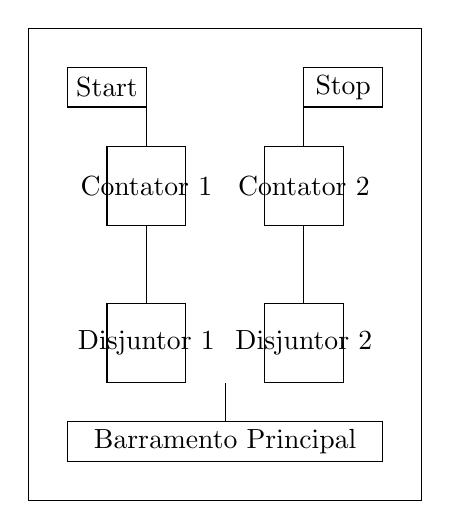
\begin{tikzpicture}[scale=0.5]
    % Caixa do quadro
    \draw (0,0) rectangle (10,12);
    % Barramento principal
    \draw (1,1) rectangle (9,2);
    \node at (5,1.5) {Barramento Principal};
    % Disjuntores
    \draw (2,3) rectangle (4,5);
    \node at (3,4) {Disjuntor 1};
    \draw (6,3) rectangle (8,5);
    \node at (7,4) {Disjuntor 2};
    % Contatores
    \draw (2,7) rectangle (4,9);
    \node at (3,8) {Contator 1};
    \draw (6,7) rectangle (8,9);
    \node at (7,8) {Contator 2};
    % Botões de comando
    \draw (1,10) rectangle (3,11);
    \node at (2,10.5) {Start};
    \draw (7,10) rectangle (9,11);
    \node at (8,10.5) {Stop};
    % Fiação
    \draw (5,2) -- (5,3);
    \draw (3,5) -- (3,7) -- (2,7);
    \draw (7,5) -- (7,7) -- (8,7);
    \draw (3,9) -- (3,11) -- (1,11);
    \draw (7,9) -- (7,11) -- (9,11);
\end{tikzpicture}

\section{Problemas e soluções}
Problema: Disparos dos dispositivos de proteção podem ser gerados pelas correntes de pico gerado ao ligar o painel. 
Solução: Escolher disjuntores com curva de disparo menos sensivel, por exemplo alterando da curva C para a curva D. 
Inicializar os circuitos sucessivamente, utilizando temporizadores auxiliares em relés de controle.\textbf{Não deve trocar o disjuntor por outro de maior capacidade pois isto pode tornar as conexões eletricas sem proteção}


%%Comum Introdução para todos os 
\chapter{Montagem }
Passo a passo de montagem...%

\input{2x2.tex}%4

\chapter{Quadro Terminal para Painel Led 2x3 ou 3x2}

Este capítulo mostra os valores efetivos para a confecção do quadro para o Painel LED Full Color. Foram usados os métodos de dimensionamento explicados no Capítulo \ref{cap:calculos}. Nas próximas seções, serão apresentados os parâmetros de projeto utilizados, a tabela de carga, os diagramas unifilar e multifilar e uma representação gráfica do quadro (esquema funcional) nas opções simples. Ao final, há uma lista de materiais para montagem.

\section{Parâmetros de projeto}

Tanto o Painel Full Color Led 2x3 quanto o Painel Full Color Led 3x2 são compostos por 6 gabinetes e deve ser alimentado com 2 cabos de força. Há três opções de resolução (P10, P8 e P5), cada uma com sua potência. A Tabela \ref{tab:pot_2x3} apresenta as informações de potência de cada gabinete, a quantidade de cabos ou grupos de até 3 gabinetes para conectar à rede elétrica e a quantidade de gabinetes e a potência total do Painel.

\begin{table}[htbp]
\caption{Potência}
\centering
\begin{tabular}{cccccc}
\toprule
\multirow{2}{*}{Item} & \multirow{2}{*}{Tipo} & \multirow{2}{*}{Potência (W)} & \multicolumn{3}{c}{Painéis} \\
\cmidrule{4-6}
& & & Cabos  & Gabinete & Potência Total (W) \\
\midrule
4 & P10 & 540 & 2 & 6 & 3240 \\
5 & P8 & 630 & 2 & 6 & 3780 \\
6 & P5 & 684 & 2 & 6 & 4104 \\
7 & P10 & 540 & 2 & 6 & 3240 \\
8 & P8 & 630 & 2 & 6 & 3780 \\
9 & P5 & 684 & 2 & 6 & 4104 \\
\bottomrule
\end{tabular}
\label{tab:pot_2x3}
\end{table}

Was this response better or worse?


\section{Tabela de Carga}
\section{Diagrama Unifilar}
\subsection{Monofásico 127 V}
\subsection{Monofásico 220 V}

\section{Diagrama Multifilar}
\subsection{Monofásico 127 V}
\subsection{Monofásico 220 V}

\section{Representação geral de disposição dos componentes no quadro terminal}

\section{Lista de materiais}
\subsection{Monofásico 127 V}
\subsection{Monofásico 220 V}

\section{Montagem do Quadro}

\subsection{Identificações e adesivos}
\begin{enumerate}
\item Identificar as fase com anilhas. Os fios de neutro serão identificados pela cor azul clara, e o aterramento por cabos de cor verde ou verde e amarelo padrão aterramento. Nos caso não possíveis a distinção por cores usar anilhas de identificação.
\item Colocar adesivos de identificação de entrada de energia e saída para o painel dos fios de fase, aterramento e neutro.
\item  Colocar adesivo de identificação do lado externo da porta, da porta.
\item Advertência no quadro como Figura \ref{fig:advQD}
\end{enumerate}


\begin{figure}[ht]
    \centering
    %\includegraphics{image/EtiqAdvQD.pdf}
    \includegraphics[scale=0.5]{image/EtiqAdvQD.pdf}
    \caption{Placa/ Adesivo de advertência para ser fixada no QD.}
    \label{fig:advQD}
\end{figure}
%e 3x2 6

\input{4x2.tex}% 8

\section{Quadro Terminal para Painel Led 3x3}
\subsection{Parametros de projeto}
\subsection{Tabela de Carga}
\subsection{Diagrama Unifilar}
\subsubsection{Monofásico 127 V}
\subsubsection{Trifásico 127/220 V}
\subsubsection{Monofásico 127 V}
\subsubsection{Trifásico 127/220 V}

\subsection{Diagrama Multifilar}
\subsubsection{Monofásico 127 V}
\subsubsection{Trifásico 127/220 V}
\subsubsection{Monofásico 127 V}
\subsubsection{Trifásico 127/220 V}

\subsection{Representação geral de disposição dos componentes no quadro terminal}

\subsection{Lista de materiais}
\subsubsection{Monofásico 127 V}
\subsubsection{Trifásico 127/220 V}
\subsubsection{Monofásico 127 V}
\subsubsection{Trifásico 127/220 V} %9

\input{5x2.tex} %10

\chapter{Quadro Terminal para Painel Led 4x3 e 6x2}

Este capítulo mostra os valores efetivos para a confecção do quadro para o Painel LED Full Color. Foram usados os métodos de dimensionamento explicados no Capítulo \ref{cap:calculos}. Nas próximas seções, serão apresentados os parâmetros de projeto utilizados, a tabela de carga, os diagramas unifilar e multifilar e uma representação gráfica do quadro (esquema funcional) nas opções simples. Ao final, há uma lista de materiais para montagem.

\section{Parâmetros de projeto}

Tanto o Painel Full Color Led 4x3 quanto o Painel Full Color Led 6x2 são compostos por 12 gabinetes e deve ser alimentado com 4 cabos de força. Há três opções de resolução (P10, P8 e P5), cada uma com sua potência. A Tabela \ref{tab:pot_4x3} apresenta as informações de potência de cada gabinete, a quantidade de cabos ou grupos de até 3 gabinetes para conectar à rede elétrica e a quantidade de gabinetes e a potência total do Painel.

\begin{table}[htbp]
\caption{Potência Painel LED 4x3 e 6x2}
\centering
\begin{tabular}{cccccc}
\toprule
\multirow{2}{*}{Item} & \multirow{2}{*}{Tipo} & \multirow{2}{*}{Potência (W)} & \multicolumn{3}{c}{Painéis} \\
\cmidrule{4-6}
& & & Cabos  & Gabinete & Potência Total (W) \\
\midrule


19 & P10 & 540 & 4 & 12 & 6480 \\
20 & P8 & 630 & 4 & 12 & 7560 \\
21 & P5 & 684 & 4 & 12 & 8208 \\


\bottomrule
\end{tabular}
\label{tab:pot_4x3}
\end{table}


\section{Tabela de Carga}
\section{Diagrama Unifilar}
\subsection{Monofásico 127 V}
\subsection{Trifásico 127/220 V}
\subsection{Monofásico 127 V}
\subsection{Trifásico 127/220 V}

\section{Diagrama Multifilar}
\subsection{Monofásico 127 V}
\subsection{Trifásico 127/220 V}
\subsection{Monofásico 127 V}
\subsection{Trifásico 127/220 V}

\section{Representação geral de disposição dos componentes no quadro terminal}

\section{Lista de materiais}
\subsection{Monofásico 127 V}
\subsection{Trifásico 127/220 V}
\subsection{Monofásico 127 V}
\subsection{Trifásico 127/220 V}

\section{Montagem do Quadro}

\subsection{Identificações e adesivos}
\begin{enumerate}
\item Identificar as fase com anilhas. Os fios de neutro serão identificados pela cor azul clara, e o aterramento por cabos de cor verde ou verde e amarelo padrão aterramento. Nos caso não possíveis a distinção por cores usar anilhas de identificação.
\item Colocar adesivos de identificação de entrada de energia e saída para o painel dos fios de fase, aterramento e neutro.
\item  Colocar adesivo de identificação do lado externo da porta, da porta.
\item Advertência no quadro como Figura \ref{fig:advQD}
\end{enumerate}


\begin{figure}[ht]
    \centering
    %\includegraphics{image/EtiqAdvQD.pdf}
    \includegraphics[scale=0.5]{image/EtiqAdvQD.pdf}
    \caption{Placa/ Adesivo de advertência para ser fixada no QD.}
    \label{fig:advQD}
\end{figure}
 %12 6x2

\chapter{Quadro Terminal para Painel Led 5x3}

Este capítulo mostra os valores efetivos para a confecção do quadro para o Painel LED Full Color. Foram usados os métodos de dimensionamento explicados no Capítulo \ref{cap:calculos}. Nas próximas seções, serão apresentados os parâmetros de projeto utilizados, a tabela de carga, os diagramas unifilar e multifilar e uma representação gráfica do quadro (esquema funcional) nas opções simples. Ao final, há uma lista de materiais para montagem.

\section{Parâmetros de projeto}

O Painel Full Color Led 5x3 é composto por 15 gabinetes e deve ser alimentado com 5 cabos de força. Há três opções de resolução (P10, P8 e P5), cada uma com sua potência. A Tabela \ref{tab:pot_5x3} apresenta as informações de potência de cada gabinete, a quantidade de cabos ou grupos de até 3 gabinetes para conectar à rede elétrica e a quantidade de gabinetes e a potência total do Painel.

\begin{table}[htbp]
\caption{Potência Painel LED 5x3}
\centering
\begin{tabular}{cccccc}
\toprule
\multirow{2}{*}{Item} & \multirow{2}{*}{Tipo} & \multirow{2}{*}{Potência (W)} & \multicolumn{3}{c}{Painéis} \\
\cmidrule{4-6}
& & & Cabos  & Gabinete & Potência Total (W) \\
\midrule


25 & P10 & 540 & 5 & 15 & 8100 \\
26 & P8 & 630 & 5 & 15 & 9450 \\
27 & P5 & 684 & 5 & 15 & 10260 \\


\bottomrule
\end{tabular}
\label{tab:pot_5x3}
\end{table}


\section{Tabela de Carga}
\section{Diagrama Unifilar}

\subsection{Trifásico 127/220 V}

\subsection{Trifásico 127/220 V}

\section{Diagrama Multifilar}

\subsection{Trifásico 127/220 V}

\subsection{Trifásico 127/220 V}

\section{Representação geral de disposição dos componentes no quadro terminal}

\section{Lista de materiais}

\subsection{Trifásico 127/220 V}

\subsection{Trifásico 127/220 V}
\section{Montagem do Quadro}

\subsection{Identificações e adesivos}
\begin{enumerate}
\item Identificar as fase com anilhas. Os fios de neutro serão identificados pela cor azul clara, e o aterramento por cabos de cor verde ou verde e amarelo padrão aterramento. Nos caso não possíveis a distinção por cores usar anilhas de identificação.
\item Colocar adesivos de identificação de entrada de energia e saída para o painel dos fios de fase, aterramento e neutro.
\item  Colocar adesivo de identificação do lado externo da porta, da porta.
\item Advertência no quadro como Figura \ref{fig:advQD}
\end{enumerate}


\begin{figure}[ht]
    \centering
    %\includegraphics{image/EtiqAdvQD.pdf}
    \includegraphics[scale=0.5]{image/EtiqAdvQD.pdf}
    \caption{Placa/ Adesivo de advertência para ser fixada no QD.}
    \label{fig:advQD}
\end{figure}

 %15

\section{Quadro Terminal para Painel Led 4x4}
\subsection{Parametros de projeto}
\subsection{Tabela de Carga}
\subsection{Diagrama Unifilar}

\subsubsection{Trifásico 127/220 V}

\subsubsection{Trifásico 127/220 V}

\subsection{Diagrama Multifilar}

\subsubsection{Trifásico 127/220 V}

\subsubsection{Trifásico 127/220 V}

\subsection{Representação geral de disposição dos componentes no quadro terminal}

\subsection{Lista de materiais}

\subsubsection{Trifásico 127/220 V}

\subsubsection{Trifásico 127/220 V} %16

\chapter{Quadro Terminal para Painel Led 7x3}

Este capítulo mostra os valores efetivos para a confecção do quadro para o Painel LED Full Color. Foram usados os métodos de dimensionamento explicados no Capítulo \ref{cap:calculos}. Nas próximas seções, serão apresentados os parâmetros de projeto utilizados, a tabela de carga, os diagramas unifilar e multifilar e uma representação gráfica do quadro (esquema funcional) nas opções simples. Ao final, há uma lista de materiais para montagem.

\section{Parâmetros de projeto}

O Painel Full Color Led 7x3 é composto por 21 gabinetes e deve ser alimentado com 7 cabos de força. Há três opções de resolução (P10, P8 e P5), cada uma com sua potência. A Tabela \ref{tab:pot_9x3} apresenta as informações de potência de cada gabinete, a quantidade de cabos ou grupos de até 3 gabinetes para conectar à rede elétrica e a quantidade de gabinetes e a potência total do Painel.



\begin{table}[htbp]
\caption{Potência Painel LED 7x3}
\centering
\begin{tabular}{cccccc}
\toprule
\multirow{2}{*}{Item} & \multirow{2}{*}{Tipo} & \multirow{2}{*}{Potência (W)} & \multicolumn{3}{c}{Painéis} \\
\cmidrule{4-6}
& & & Cabos  & Gabinete & Potência Total (W) \\
\midrule


31 & P10 & 540 & 7 & 21 & 11340 \\
32 & P8 & 630 & 7 & 21 & 13230 \\
33 & P5 & 684 & 7 & 21 & 14364 \\


\bottomrule
\end{tabular}
\label{tab:pot_7x3}
\end{table}



\section{Tabela de Carga}
\section{Diagrama Unifilar}

\subsection{Trifásico 127/220 V}

\subsection{Trifásico 127/220 V}

\section{Diagrama Multifilar}

\subsection{Trifásico 127/220 V}

\subsection{Trifásico 127/220 V}

\section{Representação geral de disposição dos componentes no quadro terminal}

\section{Lista de materiais}

\subsection{Trifásico 127/220 V}

\subsection{Trifásico 127/220 V}
\section{Montagem do Quadro}

\subsection{Identificações e adesivos}
\begin{enumerate}
\item Identificar as fase com anilhas. Os fios de neutro serão identificados pela cor azul clara, e o aterramento por cabos de cor verde ou verde e amarelo padrão aterramento. Nos caso não possíveis a distinção por cores usar anilhas de identificação.
\item Colocar adesivos de identificação de entrada de energia e saída para o painel dos fios de fase, aterramento e neutro.
\item  Colocar adesivo de identificação do lado externo da porta, da porta.
\item Advertência no quadro como Figura \ref{fig:advQD}
\end{enumerate}


\begin{figure}[ht]
    \centering
    %\includegraphics{image/EtiqAdvQD.pdf}
    \includegraphics[scale=0.5]{image/EtiqAdvQD.pdf}
    \caption{Placa/ Adesivo de advertência para ser fixada no QD.}
    \label{fig:advQD}
\end{figure}

 %21

\chapter{Quadro Terminal para Painel Led 9x3}
Este capítulo mostra os valores efetivos para a confecção do quadro para o Painel LED Full Color. Foram usados os métodos de dimensionamento explicados no Capítulo \ref{cap:calculos}. Nas próximas seções, serão apresentados os parâmetros de projeto utilizados, a tabela de carga, os diagramas unifilar e multifilar e uma representação gráfica do quadro (esquema funcional) nas opções simples. Ao final, há uma lista de materiais para montagem.

\section{Parâmetros de projeto}

O Painel Full Color Led 9x3 é composto por 27 gabinetes e deve ser alimentado com 9 cabos de força. Há três opções de resolução (P10, P8 e P5), cada uma com sua potência. A Tabela \ref{tab:pot_9x3} apresenta as informações de potência de cada gabinete, a quantidade de cabos ou grupos de até 3 gabinetes para conectar à rede elétrica e a quantidade de gabinetes e a potência total do Painel.

\begin{table}[htbp]
\caption{Potência Painel LED 9x3}
\centering
\begin{tabular}{cccccc}
\toprule
\multirow{2}{*}{Item} & \multirow{2}{*}{Tipo} & \multirow{2}{*}{Potência (W)} & \multicolumn{3}{c}{Painéis} \\
\cmidrule{4-6}
& & & Cabos  & Gabinete & Potência Total (W) \\
\midrule


34 & P8 & 630 & 9 & 27 & 17010 \\
35 & P5 & 684 & 9 & 27 & 18468 \\
36 & P10 & 540 & 9 & 27 & 14580 \\


\bottomrule
\end{tabular}
\label{tab:pot_9x3}
\end{table}


\section{Tabela de Carga}



\begin{landscape}
\begin{center}
\large\textbf{Tabela Grande}
\end{center}
\begin{tabular}{|c|c|c|c|}
%conteúdo da tabela grande
\end{tabular}
\vfill % preenche espaço vertical com espaço em branco

\begin{minipage}[t]{0.49\linewidth} % primeira coluna da parte de baixo
\centering
\large\textbf{Tabela Menor}
\begin{tabular}{|c|c|c|}
%conteúdo da tabela menor
\end{tabular}
\end{minipage}
\hfill % preenche espaço horizontal entre as colunas com espaço em branco
\begin{minipage}[t]{0.49\linewidth} % segunda coluna da parte de baixo
\centering
\large\textbf{Observações}
%conteúdo das observações
\end{minipage}

\end{landscape}

\subsection{Trifásico 127/220 V}

\begin{table}[htbp]
\centering
\caption{Tabela de Carga QT para painel Led 9x3 P10 trifásico 127/ 220V}
\resizebox{\linewidth}{!}{
\begin{tabular}{@{}llccccccccc@{}}
\toprule
Circ. & Descr. & Gab. & Polos & Potência & dist L (m) & Ib & Cabo  & DTM & DTM &  \\ 
 		&  		& P5 (Qtd) & tipo&  (W) & (m) 		& (A) & (mm²) & (A) & BCD & \\ 
 		\midrule
1 & Grupo 1 & 3 & Monofásico & 1.620 & 5 & 13 & 3 & 16 & C &  \\ 
2 & Grupo 2 & 3 & Monofásico & 1.620 & 5 & 13 & 3 & 16 & C &  \\
3 & Grupo 3 & 3 & Monofásico & 1.620 & 5 & 13 & 3 & 16 & C & \\ 
4 & Grupo 4 & 3 & Monofásico & 1.620 & 5 & 13 & 3 & 16 & C &  \\ 
5 & Grupo 5 & 3 & Monofásico & 1.620 & 5 & 13 & 3 & 16 & C &  \\ 
6 & Grupo 6 & 3 & Monofásico & 1.620 & 5 & 13 & 3 & 16 & C &  \\ 
7 & Grupo 7 & 3 & Monofásico & 1.620 & 5 & 13 & 3 & 16 & C &  \\ 
8 & Grupo 8 & 3 & Monofásico & 1.620 & 5 & 13 & 3 & 16 & C &  \\ 
9 & Grupo 9 & 3 & Monofásico & 1.620 & 5 & 13 & 3 & 16 & C &  \\ 
10 & Comunicação & 1 & Monofásico & 540 & 0 & 4 & 3 & 10 & C & \\ 
 & Geral &  & Trifásico & 15.120 & 50 & 43 & 16 & 50 & C &  \\
 \bottomrule
\end{tabular}
}
\label{tab:carga9x3T220P10}
\end{table}

\begin{table}[htbp]
\centering
\caption{Tabela de Carga QT para painel Led 9x3 P8 trifásico 127/ 220V}
\resizebox{\linewidth}{!}{
\begin{tabular}{|c|c|c|c|c|c|c|c|c|c|c|c|c|}
\hline
Circuito & Descrição & Gabinetes & Circuito & Potência & dist L (m) & \multicolumn{1}{l|}{Corrente proj} & Cabo  & DTM & DTM & FASES &  &  \\ \hline
 &  & P8 (Qtd) &  &  (W) & (m) & Ib (A) & (mm²) & (A) & Clase & \multicolumn{ 3}{c|}{R} \\ \cline{ 1- 10}
1 & Grupo 1 & 3 & Monofásico & 1.890 & 5 & 15 & 3 & 20 & C & 1.890 & 0 & 0 \\ \hline
2 & Grupo 2 & 3 & Monofásico & 1.890 & 5 & 15 & 3 & 20 & C & 0 & 1.890 & 0 \\ \hline
3 & Grupo 3 & 3 & Monofásico & 1.890 & 5 & 15 & 3 & 20 & C & 0 & 0 & 1.890 \\ \hline
4 & Grupo 4 & 3 & Monofásico & 1.890 & 5 & 15 & 3 & 20 & C & 1.890 & 0 & 0 \\ \hline
5 & Grupo 5 & 3 & Monofásico & 1.890 & 5 & 15 & 3 & 20 & C & 0 & 1.890 & 0 \\ \hline
6 & Grupo 6 & 3 & Monofásico & 1.890 & 5 & 15 & 3 & 20 & C & 0 & 0 & 1.890 \\ \hline
7 & Grupo 7 & 3 & Monofásico & 1.890 & 5 & 15 & 3 & 20 & C & 1.890 & 0 & 0 \\ \hline
8 & Grupo 8 & 3 & Monofásico & 1.890 & 5 & 15 & 3 & 20 & C & 0 & 1.890 & 0 \\ \hline
9 & Grupo 9 & 3 & Monofásico & 1.890 & 5 & 15 & 3 & 20 & C & 0 & 0 & 1.890 \\ \hline
10 & Comunicação & 1 & Monofásico & 630 & 0 & 5 & 3 & 16 & C & 630 & 0 & 0 \\ \hline
 & Geral &  & Trifásico & 17.640 & 80 & 50 & 16 & 50 & C & 6.300 & 5.670 & 5.670 \\ \hline
\end{tabular}
}
\label{tab:carga9x3T220P8}
\end{table}

\begin{table}[htbp]
\centering
\caption{Tabela de Carga QT para painel Led 9x3 P5 trifásico 127/ 220V}
\resizebox{\linewidth}{!}{
\begin{tabular}{|c|l|r|l|r|r|r|r|r|l|l|l|l|}
\hline
Circuito & \multicolumn{1}{c|}{Descrição} & \multicolumn{1}{c|}{Gabinetes} & \multicolumn{1}{c|}{Circuito} & \multicolumn{1}{c|}{Potência} & \multicolumn{1}{c|}{dist L (m)} & \multicolumn{1}{l|}{Corrente proj} & \multicolumn{1}{c|}{Cabo } & \multicolumn{1}{c|}{DTM} & \multicolumn{1}{c|}{DTM} & \multicolumn{1}{c|}{FASES} & \multicolumn{1}{c|}{} & \multicolumn{1}{c|}{} \\ \hline
 & \multicolumn{1}{c|}{} & \multicolumn{1}{c|}{P5 (Qtd)} & \multicolumn{1}{c|}{} & \multicolumn{1}{c|}{ (W)} & \multicolumn{1}{c|}{(m)} & \multicolumn{1}{c|}{Ib (A)} & \multicolumn{1}{c|}{(mm²)} & \multicolumn{1}{c|}{(A)} & \multicolumn{1}{c|}{Clase} & \multicolumn{ 3}{c|}{R} \\ \cline{ 1- 10}
1 & Grupo 1 & 3 & Monofásico & 2.052 & 5 & 16 & 3 & 20 & C & \multicolumn{1}{r|}{2.052} & 0 & 0 \\ \hline
2 & Grupo 2 & 3 & Monofásico & 2.052 & 5 & 16 & 3 & 20 & C & 0 & \multicolumn{1}{r|}{2.052} & 0 \\ \hline
3 & Grupo 3 & 3 & Monofásico & 2.052 & 5 & 16 & 3 & 20 & C & 0 & 0 & \multicolumn{1}{r|}{2.052} \\ \hline
4 & Grupo 4 & 3 & Monofásico & 2.052 & 5 & 16 & 3 & 20 & C & \multicolumn{1}{r|}{2.052} & 0 & 0 \\ \hline
5 & Grupo 5 & 3 & Monofásico & 2.052 & 5 & 16 & 3 & 20 & C & 0 & \multicolumn{1}{r|}{2.052} & 0 \\ \hline
6 & Grupo 6 & 3 & Monofásico & 2.052 & 5 & 16 & 3 & 20 & C & 0 & 0 & \multicolumn{1}{r|}{2.052} \\ \hline
7 & Grupo 7 & 3 & Monofásico & 2.052 & 5 & 16 & 3 & 20 & C & \multicolumn{1}{r|}{2.052} & 0 & 0 \\ \hline
8 & Grupo 8 & 3 & Monofásico & 2.052 & 5 & 16 & 3 & 20 & C & 0 & \multicolumn{1}{r|}{2.052} & 0 \\ \hline
9 & Grupo 9 & 3 & Monofásico & 2.052 & 5 & 16 & 3 & 20 & C & 0 & 0 & \multicolumn{1}{r|}{2.052} \\ \hline
10 & Comunicação & 1 & Monofásico & 684 & 0 & 5 & 3 & 16 & C & \multicolumn{1}{r|}{684} & 0 & 0 \\ \hline
 & Geral & \multicolumn{1}{l|}{} & Trifásico & 19.152 & 100 & 55 & 25 & 63 & C & \multicolumn{1}{r|}{6.840} & \multicolumn{1}{r|}{6.156} & \multicolumn{1}{r|}{6.156} \\ \hline
\end{tabular}
}
\label{tab:carga9x3T220P5}
\end{table}



\subsection{Trifásico 220/380 V}
\begin{table}[htbp]
\centering
\caption{Tabela de Carga QT para painel Led 9x3 P10 trifásico  220/380V}

\resizebox{\linewidth}{!}{
\begin{tabular}{|c|c|c|c|c|c|c|c|c|c|c|c|c|}
\hline
Circuito & Descrição & Gabinetes & Circuito & Potência & dist L (m) & \multicolumn{1}{l|}{Corrente proj} & Cabo  & DTM & DTM & \multicolumn{ 3}{c|}{FASES} \\ \hline
 &  & P10 (Qtd) &  &  (W) & (m) & Ib (A) & (mm²) & (A) & Clase & R & S & T \\ \hline
1 & Grupo 1 & 3 & Monofásico & 1.620 & 5 & 7 & 3 & 16 & C & 1.620 & 0 & 0 \\ \hline
2 & Grupo 2 & 3 & Monofásico & 1.620 & 5 & 7 & 3 & 16 & C & 0 & 1.620 & 0 \\ \hline
3 & Grupo 3 & 3 & Monofásico & 1.620 & 5 & 7 & 3 & 16 & C & 0 & 0 & 1.620 \\ \hline
4 & Grupo 4 & 3 & Monofásico & 1.620 & 5 & 7 & 3 & 16 & C & 1.620 & 0 & 0 \\ \hline
5 & Grupo 5 & 3 & Monofásico & 1.620 & 5 & 7 & 3 & 16 & C & 0 & 1.620 & 0 \\ \hline
6 & Grupo 6 & 3 & Monofásico & 1.620 & 5 & 7 & 3 & 16 & C & 0 & 0 & 1.620 \\ \hline
7 & Grupo 7 & 3 & Monofásico & 1.620 & 5 & 7 & 3 & 16 & C & 1.620 & 0 & 0 \\ \hline
8 & Grupo 8 & 3 & Monofásico & 1.620 & 5 & 7 & 3 & 16 & C & 0 & 1.620 & 0 \\ \hline
9 & Grupo 9 & 3 & Monofásico & 1.620 & 5 & 7 & 3 & 16 & C & 0 & 0 & 1.620 \\ \hline
10 & Comunicação & 1 & Monofásico & 540 & 0 & 2 & 3 & 16 & C & 540 & 0 & 0 \\ \hline
 & Geral &  & Trifásico & 15.120 & 90 & 25 & 6 & 32 & C & 5.400 & 4.860 & 4.860 \\ \hline
\end{tabular}
}
\label{tab:carga9x3T380P10}
\end{table}

\begin{table}[htbp]
\centering
\caption{Tabela de Carga QT para painel Led 9x3 P8 trifásico  220/380V}

\resizebox{\linewidth}{!}{
\begin{tabular}{|c|c|c|c|c|c|c|c|c|c|c|c|c|}
\hline
Circuito & Descrição & Gabinetes & Circuito & Potência & dist L (m) & \multicolumn{1}{l|}{Corrente proj} & Cabo  & DTM & DTM & FASES &  &  \\ \hline
 &  & P8 (Qtd) &  &  (W) & (m) & Ib (A) & (mm²) & (A) & Clase & \multicolumn{ 3}{c|}{R} \\ \cline{ 1- 10}
1 & Grupo 1 & 3 & Monofásico & 1.890 & 5 & 9 & 3 & 16 & C & 1.890 & 0 & 0 \\ \hline
2 & Grupo 2 & 3 & Monofásico & 1.890 & 5 & 9 & 3 & 16 & C & 0 & 1.890 & 0 \\ \hline
3 & Grupo 3 & 3 & Monofásico & 1.890 & 5 & 9 & 3 & 16 & C & 0 & 0 & 1.890 \\ \hline
4 & Grupo 4 & 3 & Monofásico & 1.890 & 5 & 9 & 3 & 16 & C & 1.890 & 0 & 0 \\ \hline
5 & Grupo 5 & 3 & Monofásico & 1.890 & 5 & 9 & 3 & 16 & C & 0 & 1.890 & 0 \\ \hline
6 & Grupo 6 & 3 & Monofásico & 1.890 & 5 & 9 & 3 & 16 & C & 0 & 0 & 1.890 \\ \hline
7 & Grupo 7 & 3 & Monofásico & 1.890 & 5 & 9 & 3 & 16 & C & 1.890 & 0 & 0 \\ \hline
8 & Grupo 8 & 3 & Monofásico & 1.890 & 5 & 9 & 3 & 16 & C & 0 & 1.890 & 0 \\ \hline
9 & Grupo 9 & 3 & Monofásico & 1.890 & 5 & 9 & 3 & 16 & C & 0 & 0 & 1.890 \\ \hline
10 & Comunicação & 1 & Monofásico & 630 & 0 & 3 & 3 & 10 & C & 630 & 0 & 0 \\ \hline
 & Geral &  & Trifásico & 17.640 & 70 & 29 & 6 & 32 & C & 6.300 & 5.670 & 5.670 \\ \hline
\end{tabular}
}
\label{tab:carga9x3T380P8}
\end{table}

\begin{landscape}
\begin{table}[htbp]
\centering
\caption{Tabela de Carga QT para painel Led 9x3 P5 trifásico  220/380V}
\begin{tabular}{|c|c|c|c|c|c|c|c|c|c|c|c|c|}
\hline
Circuito & Descrição & Gabinetes & Circuito & Potência & dist L (m) & \multicolumn{1}{l|}{Corrente proj} & Cabo  & DTM & DTM & FASES &  &  \\ \hline
 &  & P5 (Qtd) &  &  (W) & (m) & Ib (A) & (mm²) & (A) & Clase & \multicolumn{ 3}{c|}{R} \\ \cline{ 1- 10}
1 & Grupo 1 & 3 & Monofásico & 2.052 & 5 & 9 & 3 & 16 & C & 2.052 & 0 & 0 \\ \hline
2 & Grupo 2 & 3 & Monofásico & 2.052 & 5 & 9 & 3 & 16 & C & 0 & 2.052 & 0 \\ \hline
3 & Grupo 3 & 3 & Monofásico & 2.052 & 5 & 9 & 3 & 16 & C & 0 & 0 & 2.052 \\ \hline
4 & Grupo 4 & 3 & Monofásico & 2.052 & 5 & 9 & 3 & 16 & C & 2.052 & 0 & 0 \\ \hline
5 & Grupo 5 & 3 & Monofásico & 2.052 & 5 & 9 & 3 & 16 & C & 0 & 2.052 & 0 \\ \hline
6 & Grupo 6 & 3 & Monofásico & 2.052 & 5 & 9 & 3 & 16 & C & 0 & 0 & 2.052 \\ \hline
7 & Grupo 7 & 3 & Monofásico & 2.052 & 5 & 9 & 3 & 16 & C & 2.052 & 0 & 0 \\ \hline
8 & Grupo 8 & 3 & Monofásico & 2.052 & 5 & 9 & 3 & 16 & C & 0 & 2.052 & 0 \\ \hline
9 & Grupo 9 & 3 & Monofásico & 2.052 & 5 & 9 & 3 & 16 & C & 0 & 0 & 2.052 \\ \hline
10 & Comunicação & 1 & Monofásico & 684 & 0 & 3 & 3 & 10 & C & 684 & 0 & 0 \\ \hline
 & Geral &  & Trifásico & 19.152 & 60 & 32 & 10 & 32 & C & 6.840 & 6.156 & 6.156 \\ \hline
\end{tabular}
\label{tab:carga9x3T380P5}
\end{table}
\end{landscape}


\section{Diagrama Unifilar}
Apresentação dos diagramas unifilare completos para o quadro de alimentação dos paineis 9x3
As ligações do quadro são compativeis com o esquema TN-S ou TN-S-C de proteção equipotencial (aterramento). Ou seja, condutores neutro e de aterramento separados. 


\subsection{Trifásico 127/220 V}
Diagrama trifásico 127/220V P5 Figura \ref{fig:unifilar9x3220p5} - Detalhado na folha de projeto 

\begin{figure}[h]
    \centering
    \includegraphics[width=0.6\textwidth]{image/DU9X3T220P5.png}
    %\includegraphics[width=4cm]{image/EtiqAdvQD.pdf}
    \caption{Diagrama unifilar do quadro terminal para painel full color 9x3 P5 trifásico 127/220V}
   \label{fig:unifilar9x3220p5}
\end{figure}
Diagrama trifásico 127/220V P8 e P10 Figura \ref{fig:unifilar9x3220p8p10} - Detalhado na folha de projeto
\begin{figure}[h]
    \centering
    \includegraphics[width=0.6\textwidth]{image/DU9X3T220P8P10.png}
    %\includegraphics[width=4cm]{image/EtiqAdvQD.pdf}
    \caption{Diagrama unifilar do quadro terminal para painel full color 9x3 P5 trifásico 127/220V}
   \label{fig:unifilar9x3220p8p10}
\end{figure}

\subsection{Trifásico 220/380 V}
Diagrama trifásico 220/380V P5 Figura \ref{fig:unifilar9x3220p5} - Detalhado na folha de projeto
\begin{figure}[h]
    \centering
    \includegraphics[width=0.6\textwidth]{image/DU9X3T380P5.png}
    %\includegraphics[width=4cm]{image/EtiqAdvQD.pdf}
    \caption{Diagrama unifilar do quadro terminal para painel full color 9x3 P5 trifásico 127/220V}
   \label{fig:unifilar9x33800p5}
\end{figure}
Diagrama trifásico 220/380V P8 e P10 Figura \ref{fig:unifilar9x3220p8p10} - Detalhado na folha de projeto
\begin{figure}[h]
    \centering
    \includegraphics[width=0.6\textwidth]{image/DU9X3T380P8P10.png}
    %\includegraphics[width=4cm]{image/EtiqAdvQD.pdf}
    \caption{Diagrama unifilar do quadro terminal para painel full color 9x3 P5 trifásico 127/220V}
   \label{fig:unifilar9x33800p8p10}
\end{figure}

\section{Diagrama Multifilar}
Diagrama multifilar representa o esquema de ligação indicando as entradas, saídas e conexões do quadro. A seguir diagramas multifilar para as tensões entre fase 220V e 380V. Cada diagrama tem as infomações para os modulos P5, P8 e P10.
\subsection{Diagrama Multifilar do Quadro Terminal Trifásico 127/220V} 

\begin{figure}[h]
    \centering
    \includegraphics[width=\textwidth]{image/multi9x3t220.png}
    %\includegraphics[width=4cm]{image/EtiqAdvQD.pdf}
    \caption{Representação gráfica do layout interno do quadro de energia para o Painel 9x3T completo}
   \label{fig:QDTmult9x3t220}
\end{figure}

\subsection{Diagrama Multifilar do Quadro Terminal Trifásico 220/380V} 

\begin{figure}[h]
    \centering
    \includegraphics[width=\textwidth]{image/multi9x3t380.png}
    %\includegraphics[width=4cm]{image/EtiqAdvQD.pdf}
    \caption{Representação gráfica do layout interno do quadro de energia para o Painel 9x3T completo}
   \label{fig:QDTmult9x3t380}
\end{figure}


%\subsection{Trifásico 127/220 V}

%\subsection{Trifásico 220/380 V}

\section{Representação geral de disposição dos componentes no quadro terminal}
A disposição aqui é uma sugestão de layout. A disposição dos componentes poderá ser alterada conforme conveniêcia, desde o esquema de ligação elétrica do projeto não seja alterado e q ue todas as restrição/recomendações do fabricante do componente sejam atendidas.
Na figura \ref{fig:QDlayout9x3} um layout para quadro completo, indicado principalmente para exposição na área externa. 
O quadro para Painel 9x3m é composto por 10 circuitos terminais, 9 para ligar os grupos de até 3 paineis, através do cabo de força. Um circuito para as tomadas internas que tem a finalidade de alimentar o dispositivo de comunicação e controle do Painel.

Potência máxima de cada circuito terminal


\begin{figure}[h]
    \centering
    \includegraphics[width=\textwidth]{image/QD9x3tc.png}
    %\includegraphics[width=4cm]{image/EtiqAdvQD.pdf}
    \caption{Layout em escala do Quadro Terminal 9x3T completo}
   \label{fig:QDlayout9x3}
\end{figure}
%\begin{figure}[h]
%    \centering
%    \includegraphics[width=0.4\textwidth]{image/3.png}
%    %\includegraphics[width=4cm]{image/EtiqAdvQD.pdf}
%    \caption{Representação gráfica do layout interno do quadro de energia para o Painel 9x3T completo}
%   \label{fig:QDTddd}
%\end{figure}


\section{Lista de materiais}



\section{Montagem do Quadro}
\begin{itemize}
\item Qual tipo de quadro
\subitem para area externa ou interna, determina o grau de proteção dos componentes
\item Simples ou completo, determina quais componentes serão utilizados
\item ferramentas necessárias
\item  separar material necessário
\item determinar a localização dos componentes (layout)
\item fixar os componentes
\item fazer a ligação conforme projeto
\item testar
\item finalizar colocando os adesivos 
\item embalar com o manual de instalação. 

\end{itemize}

\subsection{Identificações e adesivos}
\begin{enumerate}
\item Identificar as fase com anilhas. Os fios de neutro serão identificados pela cor azul clara, e o aterramento por cabos de cor verde ou verde e amarelo padrão aterramento. Nos caso não possíveis a distinção por cores usar anilhas de identificação.
\item Colocar adesivos de identificação de entrada de energia e saída para o painel dos fios de fase, aterramento e neutro.
\item  Colocar adesivo de identificação do lado externo da porta, da porta (Figura \ref{fig:advQD_2}).
\item Fixar a Advertência na parte interna da porta do QD, como Figura \ref{fig:advQD_1}
\end{enumerate}


%\begin{figure}[ht]
%    \centering
%    %\includegraphics{image/EtiqAdvQD.pdf}
%    \includegraphics[width=4cm]{image/EtiqAdvQD.pdf}
%    \caption{Placa/ Adesivo de advertência para ser fixada na parte interna da porta do QD.}
   
%\end{figure}

\begin{figure}
\centering
\begin{subfigure}{0.4\textwidth}
	\includegraphics[width=\textwidth]{image/EtiqAdvQD.pdf}
	\caption{Advertência.}
	\label{fig:advQD_1}
\end{subfigure}
\hfill
\begin{subfigure}{0.4\textwidth}
    \includegraphics[width=\textwidth]{image/2.png}
    \caption{Risco de Choque}
    \label{fig:advQD_2}
\end{subfigure}
\caption{Placa/ Adesivo de advertência para ser fixada na porta do QD.}
\label{fig:advQD}
\end{figure}
 %27

\chapter{Quadro Terminal para Painel Led 10x4}
Este capítulo mostra os valores efetivos para a confecção do quadro para o Painel LED Full Color. Foram usados os métodos de dimensionamento explicados no Capítulo \ref{cap:calculos}. Nas próximas seções, serão apresentados os parâmetros de projeto utilizados, a tabela de carga, os diagramas unifilar e multifilar e uma representação gráfica do quadro (esquema funcional) nas opções simples. Ao final, há uma lista de materiais para montagem.

\section{Parâmetros de projeto}

O Painel Full Color Led 10x4 é composto por 40 gabinetes e deve ser alimentado com 14 cabos de força. Há três opções de resolução (P10, P8 e P5), cada uma com sua potência. A Tabela \ref{tab:pot_10x4} apresenta as informações de potência de cada gabinete, a quantidade de cabos ou grupos de até 3 gabinetes para conectar à rede elétrica e a quantidade de gabinetes e a potência total do Painel.

\begin{table}[htbp]
\caption{Potência Painel LED 10x4}
\centering
\begin{tabular}{cccccc}
\toprule
\multirow{2}{*}{Item} & \multirow{2}{*}{Tipo} & \multirow{2}{*}{Potência (W)} & \multicolumn{3}{c}{Painéis} \\
\cmidrule{4-6}
& & & Cabos  & Gabinete & Potência Total (W) \\
\midrule


37 & P8 & 630 & 14 & 40 & 25200 \\
38 & P5 & 684 & 14 & 40 & 27360 \\
39 & P10 & 540 & 14 & 40 & 21600 \\


\bottomrule
\end{tabular}
\label{tab:pot_10x4}
\end{table}

\section{Tabela de Carga}
%Para determinar a corrente de projeto, o disjuntor, a 
%Para determinar as cargas da Tabela \ref{tab:cargaT_10x4P10}, 
%a tensão de alimentação é de 220/380 V, o fatores de potência para cada circuito e geral foram 1 e 0,92 respectivamente. 
%
%
%\begin{table}[htbp]
%\centering
%\caption{Tabela de Carga QDT 10X4}
%\begin{tabular}{@{}llccccccccc@{}}
%
%\toprule
%Circuito &  &TUE &  L &  Cabo & DJ & \multicolumn{3}{c}{Fase} \\
%        & & Qtd &  (m) &  (mm²) & (A) & \\
%\midrule
%Grupo 1 & & 3 &  5 &  2,5 & 16 &  \\
%Grupo 2 & & 3 &  5 &  2,5 & 16 &  \\
%Grupo 3 & & 3 &  5 &  2,5 & 16 & \\
%Grupo 4 & &3 &  5 &  2,5 & 16 &    \\
%Grupo 5 && 3 &  5 &  2,5 & 16 &   \\
%Grupo 6 & & 3 & 5 &  2,5 & 16 &  \\
%Grupo 7 & &  3 & 5 & 2,5 & 16 &   \\
%Grupo 8 & & 3 &  5 & 2,5 & 16 &   \\
%Grupo 9 & & 3 &  5 & 2,5 & 16 &  \\
%Grupo 10 & &3 &  5 & 2,5 & 16 &    \\
%Grupo 11 & &3 &  5 & 2,5 & 16 &    \\
%Grupo 12 & &3 &  5 & 2,5 & 16 &  \\
%Grupo 13 & &2 &  5 & 2,5 & 16 &    \\
%Grupo 14 & &2 &  5 & 2,5 & 16 &    \\
%Comunicação & & 2 & 0,4 & 2,5 & 16 &  \\
%\bottomrule
%\end{tabular}
%\label{tab:cargaT_10x4P10}
%\end{table}

Neste quadro terão 14 circuitos para cada grupo de até 3 gabinetes e 1 circuito para tomadas internas utilizados na comunicação. A coluna TUE  indica a quantidade de gabinetes por grupo. Nas próximas colunas P é a potência dos equipamentos em Watts, L é o comprimento do cabo em m. Nas próximas colunas são os valores calculados para a corrente de projeto Ib, enquanto DT indica a corrente nominal do disjuntor, ambos em Ampere . Enquanto que as três últimas colunas indica a carga em  W para as fase R, fase S e Fase T.

\begin{table}[htbp]
\centering
\caption{Tabela de Carga QDT 200/380 V 10X4 T P10}

\begin{tabular}{@{}llccccccccc@{}}
%\begin{tabular}{llccccccccc}
\toprule
Circuito &  &TUE 540 & P & L & Ib & Cabo & DJ & \multicolumn{3}{c}{Fase} \\
        & & (W) & (W) & (m) & (A) & (mm²) & (A) & R & S & T \\
\midrule
Grupo 1 & & 3 & 1620 & 5 & 7,36 & 2,5 & 16 & 1620 &  &  \\
Grupo 2 & & 3 & 1620 & 5 & 7,36 & 2,5 & 16 &   & 1620 &  \\
Grupo 3 & & 3 & 1620 & 5 & 7,36 & 2,5 & 16 &   &   & 1620 \\
Grupo 4 & &3 & 1620 & 5 & 7,36 & 2,5 & 16 & 1620 &   &   \\
Grupo 5 && 3 & 1620 & 5 & 7,36 & 2,5 & 16 &   & 1620 &   \\
Grupo 6 & & 3 & 1620 & 5 & 7,36 & 2,5 & 16 &  &  & 1620 \\
Grupo 7 & &  3 & 1620 & 5 & 7,36 & 2,5 & 16 & 1620 &   &   \\
Grupo 8 & & 3 & 1620 & 5 & 7,36 & 2,5 & 16 &   & 1620 &   \\
Grupo 9 & & 3 & 1620 & 5 & 7,36 & 2,5 & 16 &   &   & 1620 \\
Grupo 10 & &3 & 1620 & 5 & 7,36 & 2,5 & 16 & 1620 &   &   \\
Grupo 11 & &3 & 1620 & 5 & 7,36 & 2,5 & 16 &   & 1620 &   \\
Grupo 12 & &3 & 1620 & 5 & 7,36 & 2,5 & 16 &   &   & 1620 \\
Grupo 13 & &2 & 1080 & 5 & 4,91 & 2,5 & 16 & 1080 &   &   \\
Grupo 14 & &2 & 1080 & 5 & 4,91 & 2,5 & 16 &   & 1080 &   \\
Comunicação & & 1 & 540 & 0,3 & 2,45 & 2,5 & 16 &  &  & 540 \\
Geral & & & 22140 & 80 & 36,61 & 10 & 10 & 7560 & 7560 & 7020 \\
\bottomrule
\end{tabular}
\label{tab:cargaT_10x4P10}
\end{table}


\subsection{Considerações}
As distribuição de paineis por grupo é uma sugestão visando uma melhor distribuição de carga nas fases.
Os tamanhos de fios de alimentação conforme parametros acima relacionados, aplicar correções quando o local de instalação tiver condições diferentes da aqui especificada.

\section{Diagrama Unifilar}

\subsection{Trifásico 127/220 V}

\subsection{Trifásico 127/220 V}

\section{Diagrama Multifilar}

\subsection{Trifásico 127/220 V}

\subsection{Trifásico 127/220 V}

\section{Representação geral de disposição dos componentes no quadro terminal}

\section{Lista de materiais}


\subsection{Trifásico 127/220 V}

\subsection{Trifásico 127/220 V}

\section{Montagem do Quadro}

\subsection{Identificações e adesivos}
\begin{enumerate}
\item Identificar as fase com anilhas. Os fios de neutro serão identificados pela cor azul clara, e o aterramento por cabos de cor verde ou verde e amarelo padrão aterramento. Nos caso não possíveis a distinção por cores usar anilhas de identificação.
\item Colocar adesivos de identificação de entrada de energia e saída para o painel dos fios de fase, aterramento e neutro.
\item  Colocar adesivo de identificação do lado externo da porta, da porta.
\item Advertência no quadro como Figura \ref{fig:advQD}
\end{enumerate}


\begin{figure}[htbp]
    \centering
    %\includegraphics{image/EtiqAdvQD.pdf}
    \includegraphics[scale=0.5]{image/EtiqAdvQD.pdf}
    \caption{Placa/ Adesivo de advertência para ser fixada no QD.}
    \label{fig:advQD}
\end{figure} %40



\chapter{Conclusão}

%\printbibliography[heading=bibintoc, title=\ebibname]

\appendix
\hyphenpenalty=10000
%\chapter{Manual de instalação do Quadro}
%%\documentclass{article}
%
\newcommand{\Linh}{9}
\newcommand{\Colun}{3}
%\title{Manual de instalação do quadro terminal}
%\author{Mundo LED}
%
%\begin{document}

%\maketitle
%%\chapter{Manual de instalação do quadro terminal}

\chapter{Manual de instalação do quadro terminal \Linh X\Colun}
%\section{introducao.tex}
Visão geral do manual e do quadro de comando. 
Lista de verificação dos materiais necessários.
Manual para instalação do Quadro Terminal para Painel Led Full Color 9 x 3 m.
\begin{figure}
\centering
\begin{subfigure}{0.4\textwidth}
	\includegraphics[width=\textwidth]{image/9.png}
	\caption{Quadro terminal para painel simples interno 9x3.}
	\label{fig:advQD_1}
\end{subfigure}
\hfill
\begin{subfigure}{0.4\textwidth}
    \includegraphics[width=\textwidth]{image/10.png}
    \caption{Quadro terminal para painel simples externo 9x3.}
    \label{fig:advQD_2}
\end{subfigure}
\begin{subfigure}{0.4\textwidth}
    \includegraphics[width=\textwidth]{image/3.png}
    \caption{Quadro terminal para painel completo externo 9x3.}
    \label{fig:advQD_2}
\end{subfigure}
\caption{Quadro terminal para painel 9x3.}
\label{fig:advQD}
\end{figure}

queda de tensão $<0,5%$


\section{Preparação do local}
O local onde ficará o quadro deve ser escolhido visando garantir a segurança e eficiência em seu funcionamento. 
O quadro terminal deverá ficará próximo ao painel em distância menor que 5 m, caso não seja possível, ajustar a distância máxima entre o quadro terminal e o quadro de distribuição geral.
A fonte de alimentação elétrica deve ser de preferencia a partir do quadro de distribuiçao geral, em circuito único e dedicado. Ou que os cabos de alimentação, as proteções esteja dimensionados obedecando as normas de segurança.
Prepare infra estrutura elétrica entre a fonte e o local onde será instalado o quadro, observando as normas de segurança.
O espaço deve ser ventilado, evitar poeira e umidade conforme o grau de proteção IPXX do quadro.
O local deve ser de fácil acesso para os eletricistas, sem obstáculos ou objetos que possam interferir na manutenção do sistema.
O quadro deve ser instalado na posição vertical, em parede resistente e ou suporte adequado para garantir sua estabilidade e segurança.
 
 \begin{quote}
 Colocar as tabelas de carga dos conjuntos de gabinete, 1, 2, 3 e comunicação
 colocar informação da divisão de carga (melhor) com quanto carga será acrescentado em cada  fase. Informação para o cliente adequar o sistema se for necessário.
 \end{quote}

%\section{Montagem do quadro de comando}
Notas sobre cabos flexiveis (fios)
Seção mínima dos cabos determinada pela norma ABNT NBR 5410. As informações aqui são orientativas, baseadas nas condições mais usuais de instalação (B1) encontradas no país.

Dimensionamento de cabos deve ser realizado conforme norma ANBT NBR 5410. Como a corrente para alimentação do painel é superior a 10 A, o quadro deve ser atendido por um circuito exclusivo.
\begin{table}[htbp]
\caption{Proteção do condutor - capacidade de condução dos condutores conforme norma ABNT NM 247-3}
\begin{tabular}{|l|l|l|}
\hline
Seção nominal &  Capacidade de condução  & Disjuntor máximo \\ \hline
1,5 mm 2  & 15,5 A  & 10 A \\ \hline
2,5 mm 2  & 21 A  & 20 A \\ \hline
4 mm 2  & 28 A  & 25 A \\ \hline
6 mm 2  & 36 A  & 32 A \\ \hline
10 mm 2  & 50 A  & 50 A \\ \hline
16 mm 2  & 68 A  & 63 A \\ \hline
25 mm 2  & 89 A  & 80 A \\ \hline
\end{tabular}
\label{tab:disjuntorcabo}
\end{table}
 


\section{Instalação do quadro de comando}
\begin{description}
\item[ATENÇÃO] Somente conectar os cabos depois do quadro devidamente fixado no local. 
\end{description}

Fixação do quadro de comando no local escolhido. 

Conexão dos cabos de entrada e saída ao quadro de comando.
\begin{description}
\item[ATENÇÃO] Primeiro conectar as saídas para o painel e depois a entrada. Trabalhar com os cabos desenergizados. 
\end{description}
 
Instalação dos dispositivos de proteção (disjuntores, fusíveis, etc.).

\section{Teste e verificação}
Verificação da conexão elétrica e aterramento.
Verificação da operação dos componentes do quadro de comando (disjuntores, contatores, etc.). 
Verificação da configuração dos ajustes de proteção e controle. Verificação da tensão e corrente elétrica.

\section{Instruções de operação e manutenção}
Instruções para a operação do quadro de comando. Instruções para a manutenção e reparação do quadro de comando. Lista de verificação de manutenção preventiva.
\begin{description}
\item[ATENÇÃO] Os dispositivos de proteção existentes no quadro não devem ser substituido por outro tipo com caracteristica diferentes.Trocar por outro dispositivo pode gerar prejuízo a vida e ao patrimônio.  Em caso de necessidade de substituição chame um profissional eletricista habilitado. 
\end{description}

\section{Conclusão}
Resumo das etapas de instalação. Informações de suporte e contato. Agradecimentos e observações finais.
\section{Definições}
Definiçoes retiradas da NBR 5410
\begin{description}
\item[Quadro de distribuição principal] Primeiro quadro de distribuição após a entrada da linha elétrica na edificação.
\end{description}






%\end{document}
%Manual de instalação para ser enviado junto com o quadro para o cliente final

Resumo das etapas de instalação. Informações de suporte e contato. Agradecimentos e observações finais.
\end{document}
